\documentclass[a4paper]{article}

\usepackage[T1]{fontenc}
\usepackage[utf8x]{inputenc}

\usepackage[a4paper]{geometry}
\geometry{verbose,tmargin=3cm,bmargin=3cm,lmargin=2cm,rmargin=2cm,headheight=2cm,headsep=1cm,footskip=2cm}

\usepackage{fancyhdr}
\usepackage{adjustbox}
\pagestyle{fancy}
\setlength{\parskip}{\medskipamount}
\setlength{\parindent}{0pt}
\usepackage{graphicx}

\makeatletter

\usepackage{float} 
\usepackage{lastpage}
\usepackage{indentfirst}

\usepackage{pgf}
\usepackage{tikz}
\usetikzlibrary{arrows,automata, shapes, positioning, calc}

\lhead[lh-even]{Edgar Vedvik (edgarmv)\\ Informatikk (BIT)}
\chead[ch-even]{TDT4205 Kompilatorteknikk\\ Problem Set 6 }
\rhead[rh-even]{\today}

\lfoot[lf-even]{}
\cfoot[cf-even]{Side \thepage{} av \pageref{LastPage}}
\rfoot[rf-even]{}

\tikzset{
    -|/.style={to path={-| (\tikztotarget)}},
    |-/.style={to path={|- (\tikztotarget)}},
}

\date{}

\makeatother

\usepackage[english]{babel}

\begin{document}


\thispagestyle{fancy}

\section{Theory}
\subsection{Control flow graphs}

\begin {enumerate}

    \item for ( a ; b ; c ) d ; e ;
        \adjustbox{valign=t}{\begin{tikzpicture}
            [->, >=stealth', auto, node distance=1cm, semithick,
            itemset/.style={rectangle, align=center, draw=black}]

            \node[itemset,minimum size=1cm] (e) {e};
            \node[itemset,minimum size=1cm] (d) [above = of e] {d};
            \node[itemset,minimum size=1cm] (b) [above = of d] {b};
            \node[itemset,minimum size=1cm] (c) [left = of b] {c};
            \node[itemset,draw,minimum size=1cm] (a) [above = of b] {a};

            \draw (a) edge (b);
            \draw (b) edge (c);
            \draw (c) edge [bend left=20] (b);
            \draw (b) edge (d);
            \draw (d) edge (e);

        \end{tikzpicture}}

    \item a ; while ( b ) \{ d ; c ; \} e ;
        \adjustbox{valign=t}{\begin{tikzpicture}
            [->, >=stealth', auto, node distance=1cm, semithick,
            itemset/.style={rectangle, align=center, draw=black}]

            \node[itemset,minimum size=1cm] (a) {a};
            \node[itemset,minimum size=1cm] (b) [below = of a] {b};
            \node[itemset,minimum size=1cm] (d) [below = of b] {d};
            \node[itemset,minimum size=1cm] (c) [left = of d] {c};
            \node[itemset,minimum size=1cm] (e) [below = of d] {e};

            \draw (a) edge (b);
            \draw (b) edge (d);
            \draw (d) edge (c);
            \draw (c) |- (b);
            \draw (b) -- +(2,0) |- (e);

          \end{tikzpicture}}

      \item a ; do \{ d ; c ; \} while ( b ); e ;
        \adjustbox{valign=m}{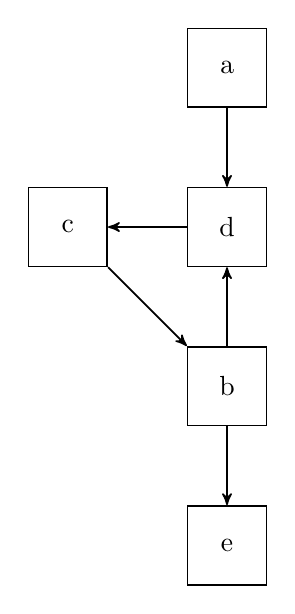
\begin{tikzpicture}
            [->, >=stealth', auto, node distance=1cm, semithick,
            itemset/.style={rectangle, align=center, draw=black}]

            \node[itemset,minimum size=1cm] (a) {a};
            \node[itemset,minimum size=1cm] (d) [below = of a] {d};
            \node[itemset,minimum size=1cm] (c) [left = of d] {c};
            \node[itemset,minimum size=1cm] (b) [below = of d] {b};
            \node[itemset,minimum size=1cm] (e) [below = of b] {e};

            \draw (a) edge (d);
            \draw (d) edge (c);
            \draw (c) edge (b);
            \draw (b) edge (d);
            \draw (b) edge (e);

          \end{tikzpicture}}
\end{enumerate}

\subsection{Optimizations}


\end{document}
